\documentclass[12pt,a4paper,oneside]{article}

\usepackage[left=1.5cm, right=1cm, top=1cm, bottom=1.5cm]{geometry}

\usepackage[utf8]{inputenc}
\usepackage[T2A]{fontenc}
\usepackage[english, russian]{babel}

\usepackage{graphicx}
\usepackage{wrapfig}
\graphicspath{ {./} }

\title{\textbf{Инструкция по сборке}}
\author{Дельта Альфа Альфа Штрих}
\date{}

\begin{document}

\maketitle

\noindent\rule{\textwidth}{1pt}

\begin{flushright}
    \textit{Штрилиц постучал в дверь 5 раз, дверь постучала в Штирлица 5 раз.\\
        — Третий закон Ньютона, — подумал Штирлиц.}
\end{flushright}

% \begin{wrapfigure}{r}{\textwidth} \centering
%     \includegraphics[width=\textwidth]{capybara} \end{wrapfigure}

\section{Установка верхней панели}
Установить TopPanel наверх (сторона с тремя отверстиями крепится на верхний
передний профиль) и закрепить её пятью DIN7985-M4 винтами с T-гайками.

\includegraphics[width=\textwidth]{toppanel}

\section{Установка кнопки}
Вставить кнопку в круглое отверстие для кнопки.

\section{Сборка камеры}
Установить CameraHolder на нижний передний профиль (центр панели должен
совпадать с центром профиля) и прикрутить её двумя DIN-7985-M4 винтами с
T-гайками. Отверстия для крепления камеры при этом должны быть выше профиля
(т.к. камера должна располагаться выше профиля), а сторона с 2 близкими
отверстиями - слева.

Нарезать M2 резьбу в трёх отверстиях для крепления камеры на CameraHolder и
прикрутить камеру пластиковыми M2x5 винтами.

Подключить камеру USB-кабелем к RPi. Начало кабеля закрепить стяжкой к профилю
(место крепления обозначено синим), остальную часть кабеля положить внутрь робота (к электронике)
так, чтобы он не торчал из робота.

\includegraphics[width=\textwidth]{usb}

\section{Сборка клешни}
Вставить ServoHolderRetainer в ServoHolder и закрепить их DIN-7985-M3 винтом
длиной 12 мм с гайкой DIN-934-M3.

\includegraphics[width=\textwidth]{servoholder}

Вставить получившуюся конструкцию в TopPanel и закрептить DIN-7985-M3 винтами
длиной 12 мм с гайками DIN-934-M3.

\includegraphics[width=\textwidth]{servoholder-toppanel}

Вставить сервопривод MG995 в ServoHolder так, чтобы вращающаяся часть была
направлена вправо и находилась ближе к переду робота (см. рисунок) и закрепить
его четырьмя DIN-7985-M4 винтами длиной 8 мм с DIN-934-M4 гайками (гайки должны
находиться слева, чтобы винты не мешали движению клешни).

\includegraphics[width=\textwidth]{installedservo}

Провод сервопривода закрепить резинкой в обведённом красным цветом месте.

\includegraphics[width=\textwidth]{servowires}

Прикрутить крестовую насадку сервопривода к Claw (клешне) 8 саморезами DIN-7986.

\includegraphics[width=\textwidth]{servo}

Повернуть сервопривод в крайнее положение против часовой стрелки (если руками
это сделать сложно, можно использовать какую-либо насадку).

Присоеденить клешню к сервоприводу так, чтобы в крайнем положении против часовой
стрелки сервопривода клешня была в нижнем положении (касалась верхней панели
робота).

\includegraphics[width=\textwidth]{full_claw}

\section{Электронные компоненты}
Отрезать черный и красный HB4 провода длиной около 30 см.

Выбрать пару замыкаемых на кнопке контактов (у нас нет этих кнопок, поэтому мы
не знаем, какие именно контакты замыкаются) и припаять к ним 2 провода. Вторые
концы этих проводов обжать в разъёме XHP-5 - красный в 5, чёрный в 2 (см.
рисунок) и подключить его к разъёму RNG8 робота (отмечен зелёным).

\includegraphics[width=0.3\textwidth]{buttoncontacts}

Провод от сервопривода подключить в разъём D44 робота (отмечен красным) так,
чтобы жёлтый провод был подключен к S. Если длины штатного провода не хватит,
воспользоваться сервоудлиннителями.

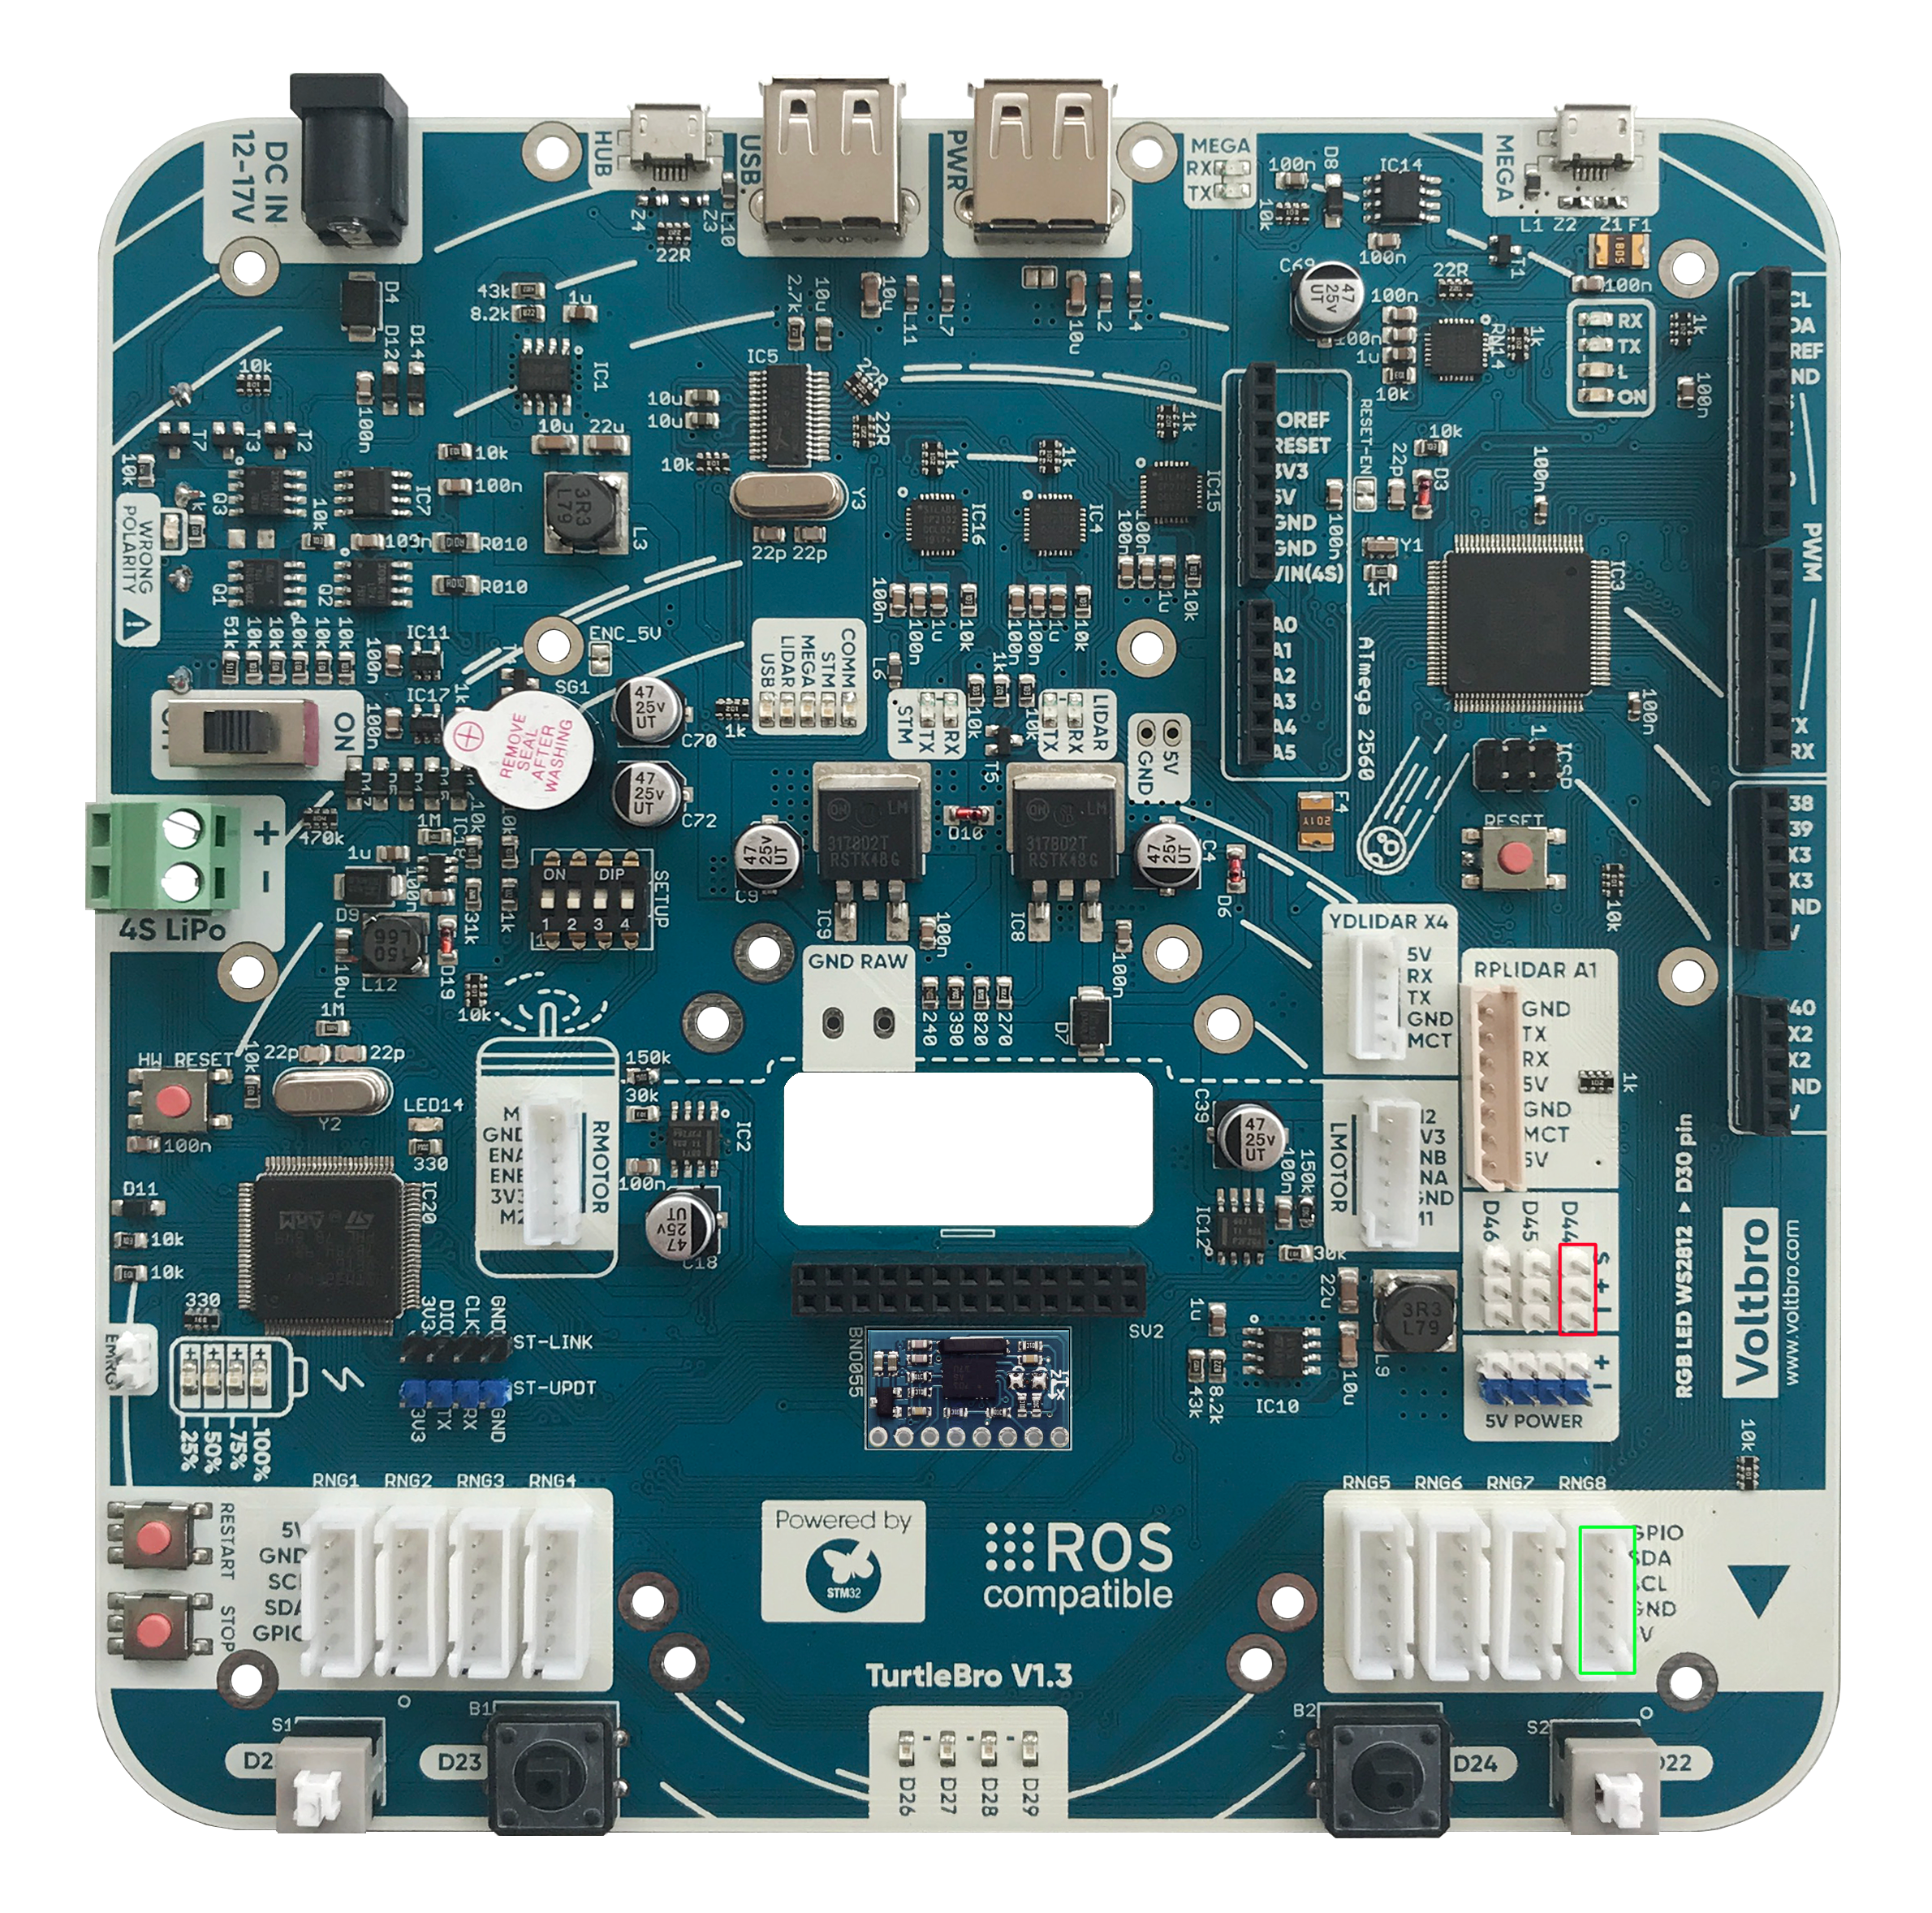
\includegraphics[width=\textwidth]{pins}

Схема электроники находится в файле electro.pdf.

После выполнения всех тестов прошить скетч controller.

\section{Тесты}
Описание порядка тестирования находится в файле tests.pdf.

\newpage

\begin{figure}
\centering
\includegraphics[width=0.9\textwidth]{capybara.jpg}
\caption{\label{fig:capybara}Капибара.}
\end{figure}

\end{document}
